Certainly! Below is a TikZ LaTeX code to generate diagrams representing the UO invariants at order \((1,1)\) for \(n=1\), \(n=2\), and \(n=3\). Each set of diagrams is labeled accordingly, and note that sets like (B2 and B3), (C2 and C3), and (C4 and C5) are considered indistinguishable in the pure orthogonal case.

```latex
\documentclass[tikz,border=5]{standalone}
\usetikzlibrary{shapes.geometric, arrows.meta}

\tikzset{
    block/.style={rectangle, draw=black, fill=white!20, text width=6em, text centered, rounded corners, minimum height=4em},
    line/.style={thick,->,>=stealth'},
    decision/.style={diamond, draw=black, fill=white!20, text width=4em, text badly centered, node distance=3cm, inner sep=0pt}
}

\begin{document}

% Diagram A: n=1
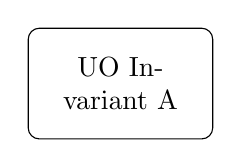
\begin{tikzpicture}[node distance=2cm]
    \node [block] (A) {UO Invariant A};
\end{tikzpicture}

% Diagram B1: n=2
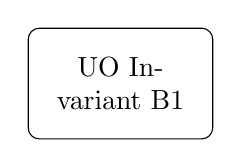
\begin{tikzpicture}[node distance=2cm]
    \node [block] (B1) {UO Invariant B1};
\end{tikzpicture}

% Diagram B2: n=2 (indistinguishable from B3)
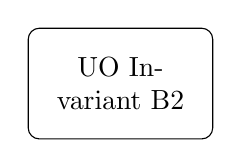
\begin{tikzpicture}[node distance=2cm]
    \node [block] (B2) {UO Invariant B2};
\end{tikzpicture}

% Diagram C1: n=3
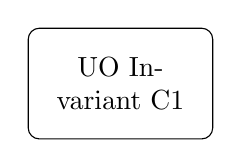
\begin{tikzpicture}[node distance=2cm]
    \node [block] (C1) {UO Invariant C1};
\end{tikzpicture}

% Diagram C2: n=3 (indistinguishable from C3)
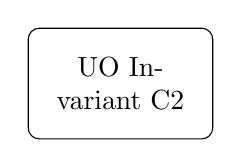
\begin{tikzpicture}[node distance=2cm]
    \node [block] (C2) {UO Invariant C2};
\end{tikzpicture}

% Diagram C4: n=3 (indistinguishable from C5)
\begin{tikzpicture}[node distance=2cm]
    \